\documentclass[]{article}
\usepackage{amsmath}
\usepackage{graphicx}
%\usepackage{xcolor}
\usepackage{hyperref}
\usepackage[dvipsnames]{xcolor}
\usepackage{matlab-prettifier}
\usepackage{fullpage}

\graphicspath{ {images/} }

% Title Page
\title{Laboratory 5: Rigid and Non-Rigid Structure from Motion}
\author{Jesus Miguel Adrian Matos}
\date{\today}


\begin{document}
\maketitle

\begin{abstract}
\noindent 
The aim of this laboratory concerns on rigid and non-rigid structure from motion, by completing a Matlab code provided previously. 

\noindent In particular, the report is divided as follows:
\begin{itemize}
\item Section 1: we explain the inputs in order to define the motion structure.
\item Section 2: we compute the structure if the results, that is the shape of the matrix
\item Section 3: we explain the code to compute the rigid structure from motion by factorization.
\item Section 4: we explain the code to compute the non-Rigid structure from motion by non-linear optimization and assuming a low- rank shape model.
\item Section 5: we explain the code to compute the non-Rigid structure from motion by factorization and assuming a low-rank trajectory model.
\end{itemize}
%con los conocimientos de clase
%En la parte 1 explicamos las entradas para poder conseguir la estructura de movimiento. 
%En la parte 2 calculamos la estructura del resultado, que es la forma de la matriz. 
%
%using Matlab software y los conocimientos de clase
%En la parte 3 explicamos el codigo para calcular la estructura para un cuerpo Rigid structure from motion by factorization.
%En la parte 4 explicamos el codigo para calcular la estructura para un cuerpo Non-Rigid structure from motion by non-linear optimization and assuming a low- rank shape model.
%En la parte 5 explicamos el codigo para calcular la estructura para un cuerpo Non-Rigid structure from motion by factorization and assuming a low-rank trajectory model.


\end{abstract}

%\newpage 

\section{Inputs:}
Given an image in the frame $k$, calling $p$ as the number of track point and $f$ as the number of frames, then the image is described by a $2\times p$ matrix $I_k$, defined

\begin{equation}
I_{k}=
\begin{pmatrix}
x_{1} & x_{2} & \cdots & x_{p}\\
y_{1} & y_{2} & \cdots & y_{p}
\end{pmatrix}
\end{equation}
where $(x_k,y_k)$ are the coordinated of the bidimensional space.
As a consequence, the input matrix is expressed

\begin{equation}
Input=
\begin{pmatrix}
I_{1}\\
I_{2}\\
\vdots\\
I_{f}\\
\end{pmatrix}
\end{equation}
\section{Outputs:}
We want to obtain a representation in the 3D plane of the points tracked in the 2D images. The resulting matrix is

\begin{equation}
Output=
\begin{pmatrix}
x_{1} & x_{2} & \cdots & x_{p}\\
y_{1} & y_{2} & \cdots & y_{p}\\
z_{1} & z_{2} & \cdots & z_{p}
\end{pmatrix}
\end{equation}
Where $(x,y,z)$ represents the 3D coordinates in the $\Re^{3}$ space.
\section{First Part (Rigid structure from motion by factorization)}
\noindent In this task, factorization for a rigid body must be implemented, as shown in the following slide figure \ref{fig:slideT1}.
\noindent So, we should complete the orthogonal factorization function by means of the file \textbf{rigidfactorization ortho.m}. The completed code runs with a provided test data composed by a synthetic sequence with an Ogre face, and the 3D reconstruction error is reported.\\

\begin{figure}[h]
    \centering
    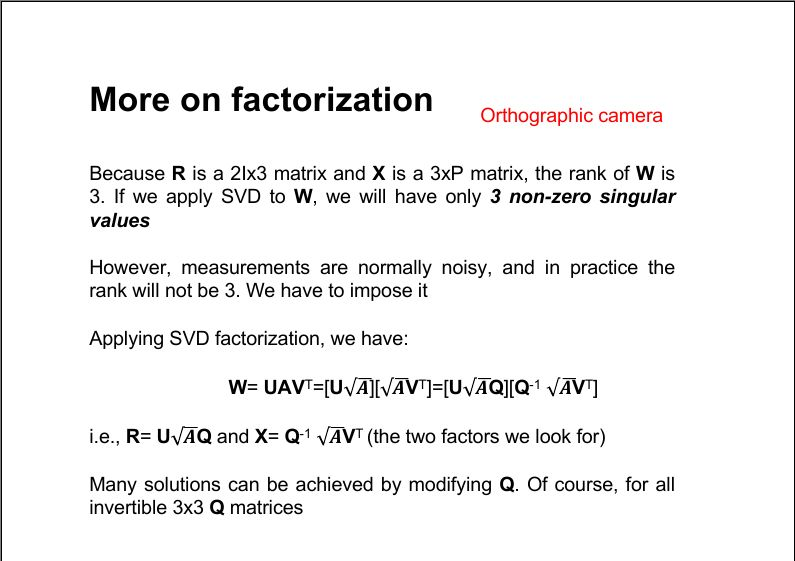
\includegraphics[width=0.75\textwidth]{T1/slide}
    \caption{Factoring slide}
    \label{fig:slideT1}
\end{figure}

\subsection{Code:}
\noindent Now, we introduce the code \ref{lst:codeT1}. We will explain each line number:\\ 
\noindent For the line $1$ and $2$, $Zc$ is defined as the difference between the input matrix and the average of all the points in each frame, and not as the input matrix.
This way, we no longer have to consider translation in the computations.\\ 
\noindent Therefore, the average matrix would be the following, with dimensions $2f\times p$
\begin{equation}\label{eq:mean}
Mean=
\begin{pmatrix}
Mean_{1} & Mean_{1} & \cdots Mean_{1}\\
Mean_{2} & Mean_{2} & \cdots Mean_{2}\\
\vdots & \vdots & \ddots & \vdots\\
Mean_{f} & Mean_{f} & \cdots Mean_{f}
\end{pmatrix}
\end{equation}
\noindent where
\begin{equation}
Media_{k}=
\begin{pmatrix}
\frac{x_{1} + x_{2} + \cdots + x_{p}}{p}\\
\frac{y_{1} + y_{2} + \cdots + y_{p}}{p}
\end{pmatrix}
\end{equation}
\noindent for any $k$ between $1$ and $f$.
\noindent Therefore from \ref{eq:mean} we have:
\begin{equation}
Zc=Input-Mean
\end{equation}

\noindent In the line "$3$, we calculate the factorization called Singular Value Decomposition (SVD).\\
\noindent In the line $4$ and $5$, we approximate $R=U(:,1:3)D(1:3, 1:3)^{1/2}$ and $S=D(1:3, 1:3)^{1/2}V(:, 1:3)'$ (where $R$ represents rotation and $S$ represents shape). Knowing that the rank of $RS$ is 3, therefore the truth mathix $D$ should have a dimension of $3\times 3$, then we do the following:\\
\begin{itemize}
\item $D$: We take the first 3 rows and the first 3 columns.
\item $U$: We take only the first 3 columns.
\item $V$: We take only the first 3 columns.
\end{itemize}
\noindent therefore in that way we can calculate $S$ as $U_{2I\times 3}\sqrt{D}_{3\times 3}$ and R as $\sqrt{D}_{3\times 3}V^{'}_{3\times 3I}$\\

\noindent In the ``while loop" of the line $10$, we try to reduce $\Vert Zc-RU\Vert$  to the threshold, which in the code is called epsilon. The idea to optimize the rotation matrix is use the rotation condition $R_{i}R_{i}'=I$, where $I$ corresponds to the identity matrix. This rotation condition is used to calculate $T$ in the code and thus be able to calculate the new matrices $S$ and $R$.

\begin{lstlisting}[style=Matlab-editor, numbers=left,label={lst:codeT1},captionpos=b, caption={Factorization code for orthographic camera}]
T = mean(Zc,2);
Zc = Zc - repmat(T,1,size(Zc,2)); 
[U, D, V] = svd(Zc);
R = U(:, 1:3)*(D(1:3, 1:3) ^ 1/2); 
S = (D(1:3, 1:3) ^ 1/2)*V(:, 1:3)';
% Metric Upgrade Step
F=size(Zc,1);
k=0;
thenorm=epsilon+1;
while thenorm>epsilon && k<n_iter
    Rp=R;
    M=[];
    for f=1:2:F
       Rf=R(f:f+1,:);
       [U2,useless,V2]=svd(Rf,'econ');       
       T=U2*V2';
       M=[M;T(1:2,:)];
   end 
    S=pinv(M)*Zc;
    R=Zc*pinv(S);
    k=k+1;
    thenorm=norm(R-Rp,'fro')/numel(M);
end
\end{lstlisting}
\noindent Finally, ones that the optimization finish, we obtain a shape matrix $S$ to compare as the truth matix shape $X$.

\subsection{Examples:}
\noindent Here we will show how to reconstruct the face of an Ogre with the given frames and using the following input parameters:

\begin{itemize}
\item threholder: $10^{-7}$
\item maximum number of iterations: 200
\end{itemize}

\begin{figure}[h]
    \centering
    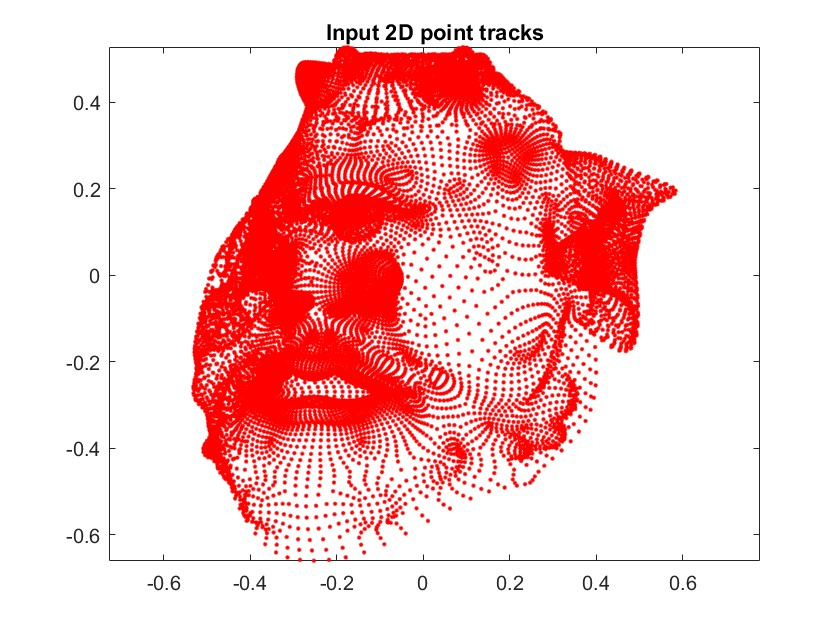
\includegraphics[width=0.6\textwidth]{T1/figure1}
    \caption{The original face of the Ogre.}
    \label{fig:real_ogre}
\end{figure}

\begin{figure}[h]
    \centering
    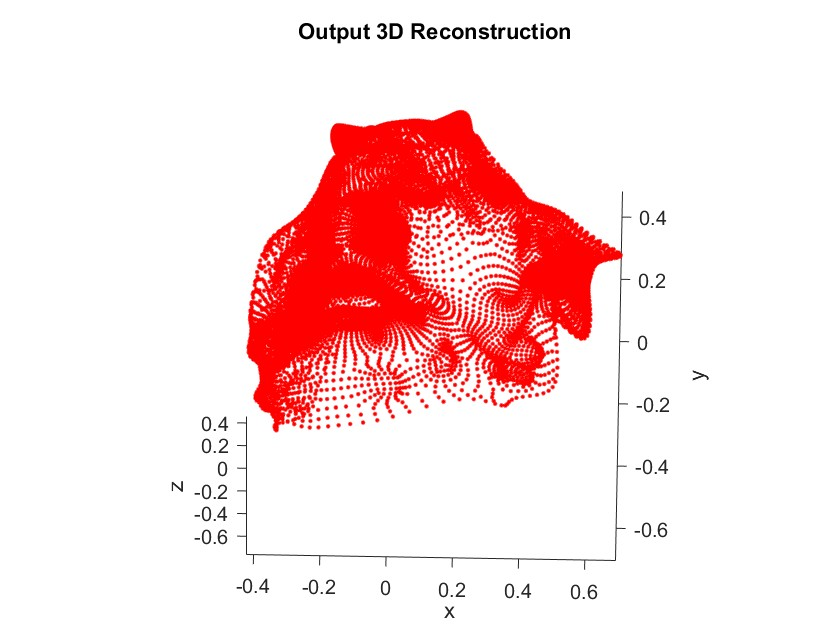
\includegraphics[width=0.75\textwidth]{T1/figure3}
    \caption{The Ogre's face reconstructed by the algorithm.}
    \label{fig:ogre}
\end{figure}

\begin{figure}[h!]
    \centering
    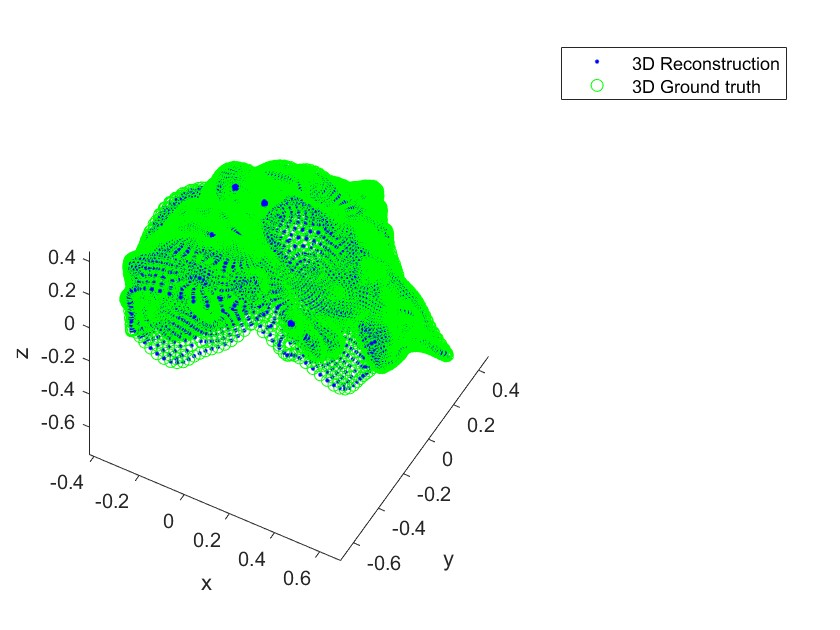
\includegraphics[width=0.75\textwidth]{T1/figure2}
    \caption{Comparison between the 3D representation of the Ogre's original face and its face reconstructed by the algorithm.}
    \label{fig:real_ogre_vs_ogre}
\end{figure}
\noindent As can be seen in Figure \ref{fig:real_ogre_vs_ogre}, the reconstruction of the Ogre's face is quite good. This is demonstrated by the fact that the error between the original Ogre's face and its face reconstructed by the algorithm is 0,0026993\% it means quite low, as depicted Figure \ref{fig:3d_error}.

\begin{figure}[h!]
    \centering
    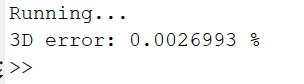
\includegraphics[width=0.4\textwidth]{T1/3derror}
    \caption{Error between the ogre's face and the reconstructed face.}
    \label{fig:3d_error}
\end{figure}

\section{Second Part (Non-Rigid structure from motion by non-linear optimization and assuming a low-rank shape model)}
\noindent In this task we should perform a nonlinear optimization for a non-rigid body, assuming a low rank. This code uses Levenberg-Marquardt algorithm to optimize the non-linear equation that it is shown to next:
\begin{equation}\label{eq:optimization}
	\underset{R^{i},B_{k},l_{i}^{k},t^{i}}{\arg\min}
	\sum_{i=1}^{i}\Vert \widehat{W}^{i}-R^{i}\sum_{k=1}^{k}l_{i}^{k}B_{k}-t^{i}\Vert^{2}+
	\gamma\sum_{i=1}^{i-1}\Vert L^{i}-L^{i+1} \Vert^{2}+
	\phi\sum_{i=1}^{i-1}\Vert R^{i}-R^{i+1} \Vert^{2}
\end{equation}
\noindent Where:
$B_{k}$ is a row of bases matrix.
$R^{i}$ is a rotation for a point in matrix column $i$ of $X$, which is the 3D shape vector. 
$l_{i}$ are the constants such that $\sum_{k=1}^{k}l_{i}^{k}B_{k}=X$.
$t^{i}$ is the translation.
$L^{i}$ is the vector of all constants in frame $i$.
\noindent The norm used is the Frobenius norm.\\

\noindent In order to calculate the Levenberg-Marquardt optimization, we need to calculate the Jacobian form of the equation \ref{eq:optimization}. We do this as shown in the following slide Figure \ref{fig:slideT2}

\begin{figure}[h]
	\centering
	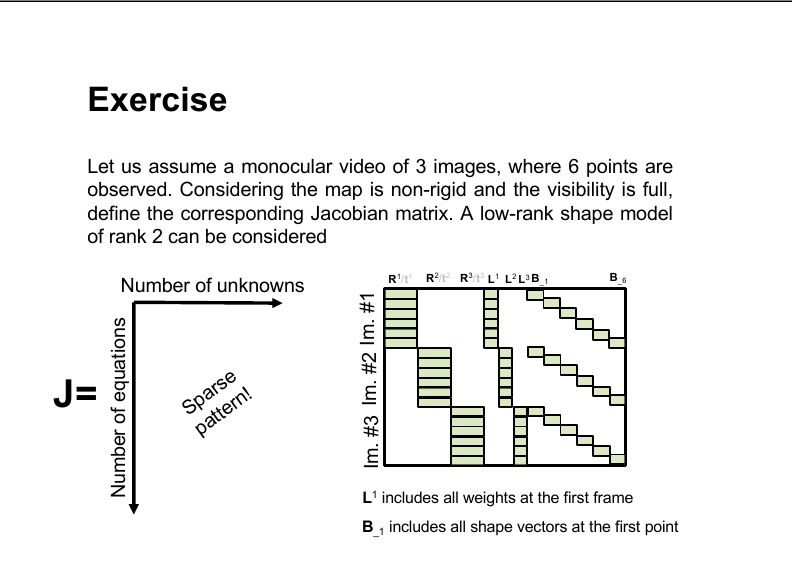
\includegraphics[width=0.7\textwidth]{T2/slide}
	\caption{Jacobian form}
	\label{fig:slideT2}
\end{figure}

\subsection{Code:}
\noindent Now we will show how this Jacobian form is calculated in the code.\\

\noindent So first we will define the dimensions of Jacobian matrix. For this code we are using quaternions for the rotations, therefore $R^{i}$ is $2\times 4$.\\

\noindent Then the dimension of Jacobian matrix is defined in the following way

\begin{itemize}
	\item number of rows of $Dim(J^{rows})=$
	\textcolor{green}{$2\sum_{i=1}^{f}(number of points visible in frame i)$}
	\item number of columns of $Dim(J_{columns})=$
	\textcolor{red}{$4f$}$+$
	\textcolor{blue}{$2f$}$+$
	\textcolor{orange}{$kf$}$+$
	\textcolor{Yellow}{$3kp$}	
\end{itemize}

\noindent Where $f$ is the number of frames, $p$ is the total number of points tracked and $k$ is the total number of bases.\\

\noindent \textbf{Explaining row sizes:}\\
\noindent \textbf{\textcolor{green}{Green}:} Represents the visible points per frame. When we multiply the sum of the visible points by two it is because the rotations are in quaternions. The quaternions are 2x4 and then they are two vectors per each point and that is why it is multiplied by two.\\ 

\noindent \textbf{Explaining column sizes:}\\

\noindent \textbf{\textcolor{red}{Red}:} Represents the value of the columns of the rotation matrix, which is $2\times 4$ quaternions. We have a rotation matrix $R^{i}$ for each frame $i$. Therefore, the dimension is $4f$, where $f$ is the number of frames.\\ 
%aquimequedeNatalia%

\noindent \textbf{\textcolor{blue}{Blue}:} Represents the translation matrix $t^{i}$, whose dimension is $1\times 2$, for each frame $i$, therefore $2f$ where $f$ is the number of frames.\\

\noindent \textbf{\textcolor{orange}{Orange}:} Represents the matrix $L_{i}$ whose dimension is $1\times k$ for each frame $i$, therefore $kf$ where $f$ is the number of frames.\\

\noindent \textbf{\textcolor{lime}{Yellow}:} Represents the matrix $B_{b}$ whose dimension is $3\times p$ for each base $b$, therefore $3pk$ where $k$ is the number of bases.\\

\noindent Well then we need to define the shape of our Jacobian matrix by putting $1$ where there are values and leaving $0$ in the spaces that do not exist, as shown in the following code.\\

\begin{lstlisting}[style=Matlab-editor, numbers=left]
for i=1:n_frames
        for j=1:nnz(vij(i,:))        
            J(2*j-1+computed_points:2*j+computed_points,6*j-5:6*j)=ones(2,6);
            J(2*j-1+computed_points:2*j+computed_points,K*j-K+1+6*n_frames:K*j+6*n_frames)=ones(2,K);
            J(2*j-1+computed_points:2*j+computed_points,3*K*j-3*K+1+(6+K)*n_frames:3*K*j+(6+K)*n_frames)=ones(2,3*K);
        end
        computed_points=computed_points+2*nnz(vij(i,:));
    end
\end{lstlisting}
\noindent In the first for loop each frame is iterated, in the second for loop only the points visible in that frame are iterated.\\
\begin{lstlisting}[style=Matlab-editor]
J(2*j-1+computed_points:2*j+computed_points,6*j-5:6*j)=ones(2,6);
\end{lstlisting}
\noindent Here, the Jacobian is calculated for the rotation $R$ part (in quaternions) and the translation part $t$, having this
\begin{equation}
\begin{pmatrix}
R_{2\times 4} & | & t_{2\times 2}
\end{pmatrix}_{2\times 6}
\end{equation}
we can add a matrix of ones of $2\times 6$

\noindent Now, the Jacobian is calculated for the constants $L^{i}$ part, where $L^{i}=[l_{1}^{i},l_{2}^{i}, \cdots, l_{k}^{i}]$ such that $i$ is a frame.
\begin{lstlisting}[style=Matlab-editor]
J(2*j-1+computed_points:2*j+computed_points,K*j-K+1+6*n_frames:K*j+6*n_frames)=ones(2,K);
\end{lstlisting}
and for that, in the code is added a matrix of ones from $2\times k$.\\

\noindent Now, the Jacobian is calculated for the bases $B_{i}$ part, where
\begin{equation}
B_{i}=\begin{pmatrix}
[b_{1}^{i}]_{3\times 1} & [b_{2}^{i}]_{3\times 1} & \cdots & [b_{k}^{i}]_{3\times 1}
\end{pmatrix}_{3\times k}
\end{equation}
\begin{lstlisting}[style=Matlab-editor]
J(2*j-1+computed_points:2*j+computed_points,3*K*j-3*K+1+(6+K)*n_frames:3*K*j+(6+K)*n_frames)=ones(2,3*K);
\end{lstlisting}
\noindent and for that, in the code is added a matrix of ones from $2\times 3k$.\\

\noindent Now we calculate the Jacobian part of the priors.\\
\begin{equation}\label{eq:priors}
\underset{R^{i},B_{k},l_{i}^{k},t^{i}}{\arg\min}
\gamma\sum_{i=1}^{i-1}\Vert L^{i}-L^{i+1} \Vert^{2}+
\phi\sum_{i=1}^{i-1}\Vert R^{i}-R^{i+1} \Vert^{2}
\end{equation}
\noindent from the equation we have
\begin{itemize}
\item \textbf{The prior with respect to the rotation $R^{i}$:} This means that the rotation between two consecutive frames $\sum_{i=1}^{i-1}\Vert L^{i}-L^{i+1} \Vert^{2}$ do not have abrupt changes, it is a smoothing of the rotations.
\item \textbf{The prior with respect to the constants $L^{i}$:} This means that the costates that multiply the bases, such that $X^{i}=\sum_{j=1}^{k}l^{i}_{j}B_{j}$ form the shape matrix. Therefore, if the constans for two consecutive frames $\sum_{i=1}^{i-1}\Vert L^{i}-L^{i+1} \Vert^{2}$ does not have abrupt changes then the shapes do not have abrupt changes, it is a smoothing of the shapes.
\end{itemize}

\noindent Well, we use the expressions in equation \ref{eq:priors} to calculate the dimension of the Jacobian for the priors.\\

\noindent So from this equation \ref{eq:priors} and the orange color of the equation \ref{eq:optimization} we deduce that the Jacobian dimension for the prior L would be 
\begin{equation}
Dim(J_{rows})=f-1
Dim(J_{columns})=kf
\end{equation}
\noindent and the blue and red color of the equation \ref{eq:optimization} also we can deduce the Jacobian dimension for the prior R as
\begin{equation}
Dim(J_{rows})=f-1
Dim(J_{columns})=6f
\end{equation}

\noindent Now we will show how we fill the indices that have a value in the Jacobian Matrix of the $L$ prior with 1 and otherwise hold with zero.\\
\begin{lstlisting}[style=Matlab-editor]
if (priors.coeff_prior == 1)
     % prior terms on L
     L=spalloc(n_frames-1,(K+6)*n_frames + K*3*n_points,2*K*(n_frames-1));     
     for i=1:n_frames-1
        L(i,K*i-K+1+6*n_frames:K*i+K+6*n_frames)=ones(1,2*K);        
     end
     if K==1
         J(2*nnz(vij)+1:size(J,1), :)=L;
     else
         J(2*nnz(vij)+1:2*nnz(vij)+n_frames-1, :)=L;
     end
 end 
\end{lstlisting}
\noindent We do the following, we take the $L_{i}$ and $L_{i+1}$ and join them as shown in the equation \ref{eq:Li_li1}
\begin{equation}\label{eq:Li_li1}
\begin{pmatrix}
[L_{i}]_{1\times k} & | & [L_{i+1}]_{1\times k}
\end{pmatrix}_{1\times 2k}
\end{equation}
\noindent and because of this in the code we add a matrix of ones $1\times 2K$.\\
\noindent For the Jacobian Matrix of the $R$ prior is the similar way, in this case we joint $R^{i}$ and $R^{i+1}$ like show in the equation \ref{eq:Ri_Ri1}
\begin{equation}\label{eq:Ri_Ri1}
\begin{pmatrix}
[R^{i}]_{1\times 6} & | & [R_{i+1}]_{1\times 6}
\end{pmatrix}_{1\times 12}
\end{equation}
\noindent and because of this in the code we add a matrix of ones $1\times 12$.\\
Joining the Jacobian and the Jacobian of the priors we have the following graph figure \ref{fig:J}.

\begin{figure}[h]
    \centering
    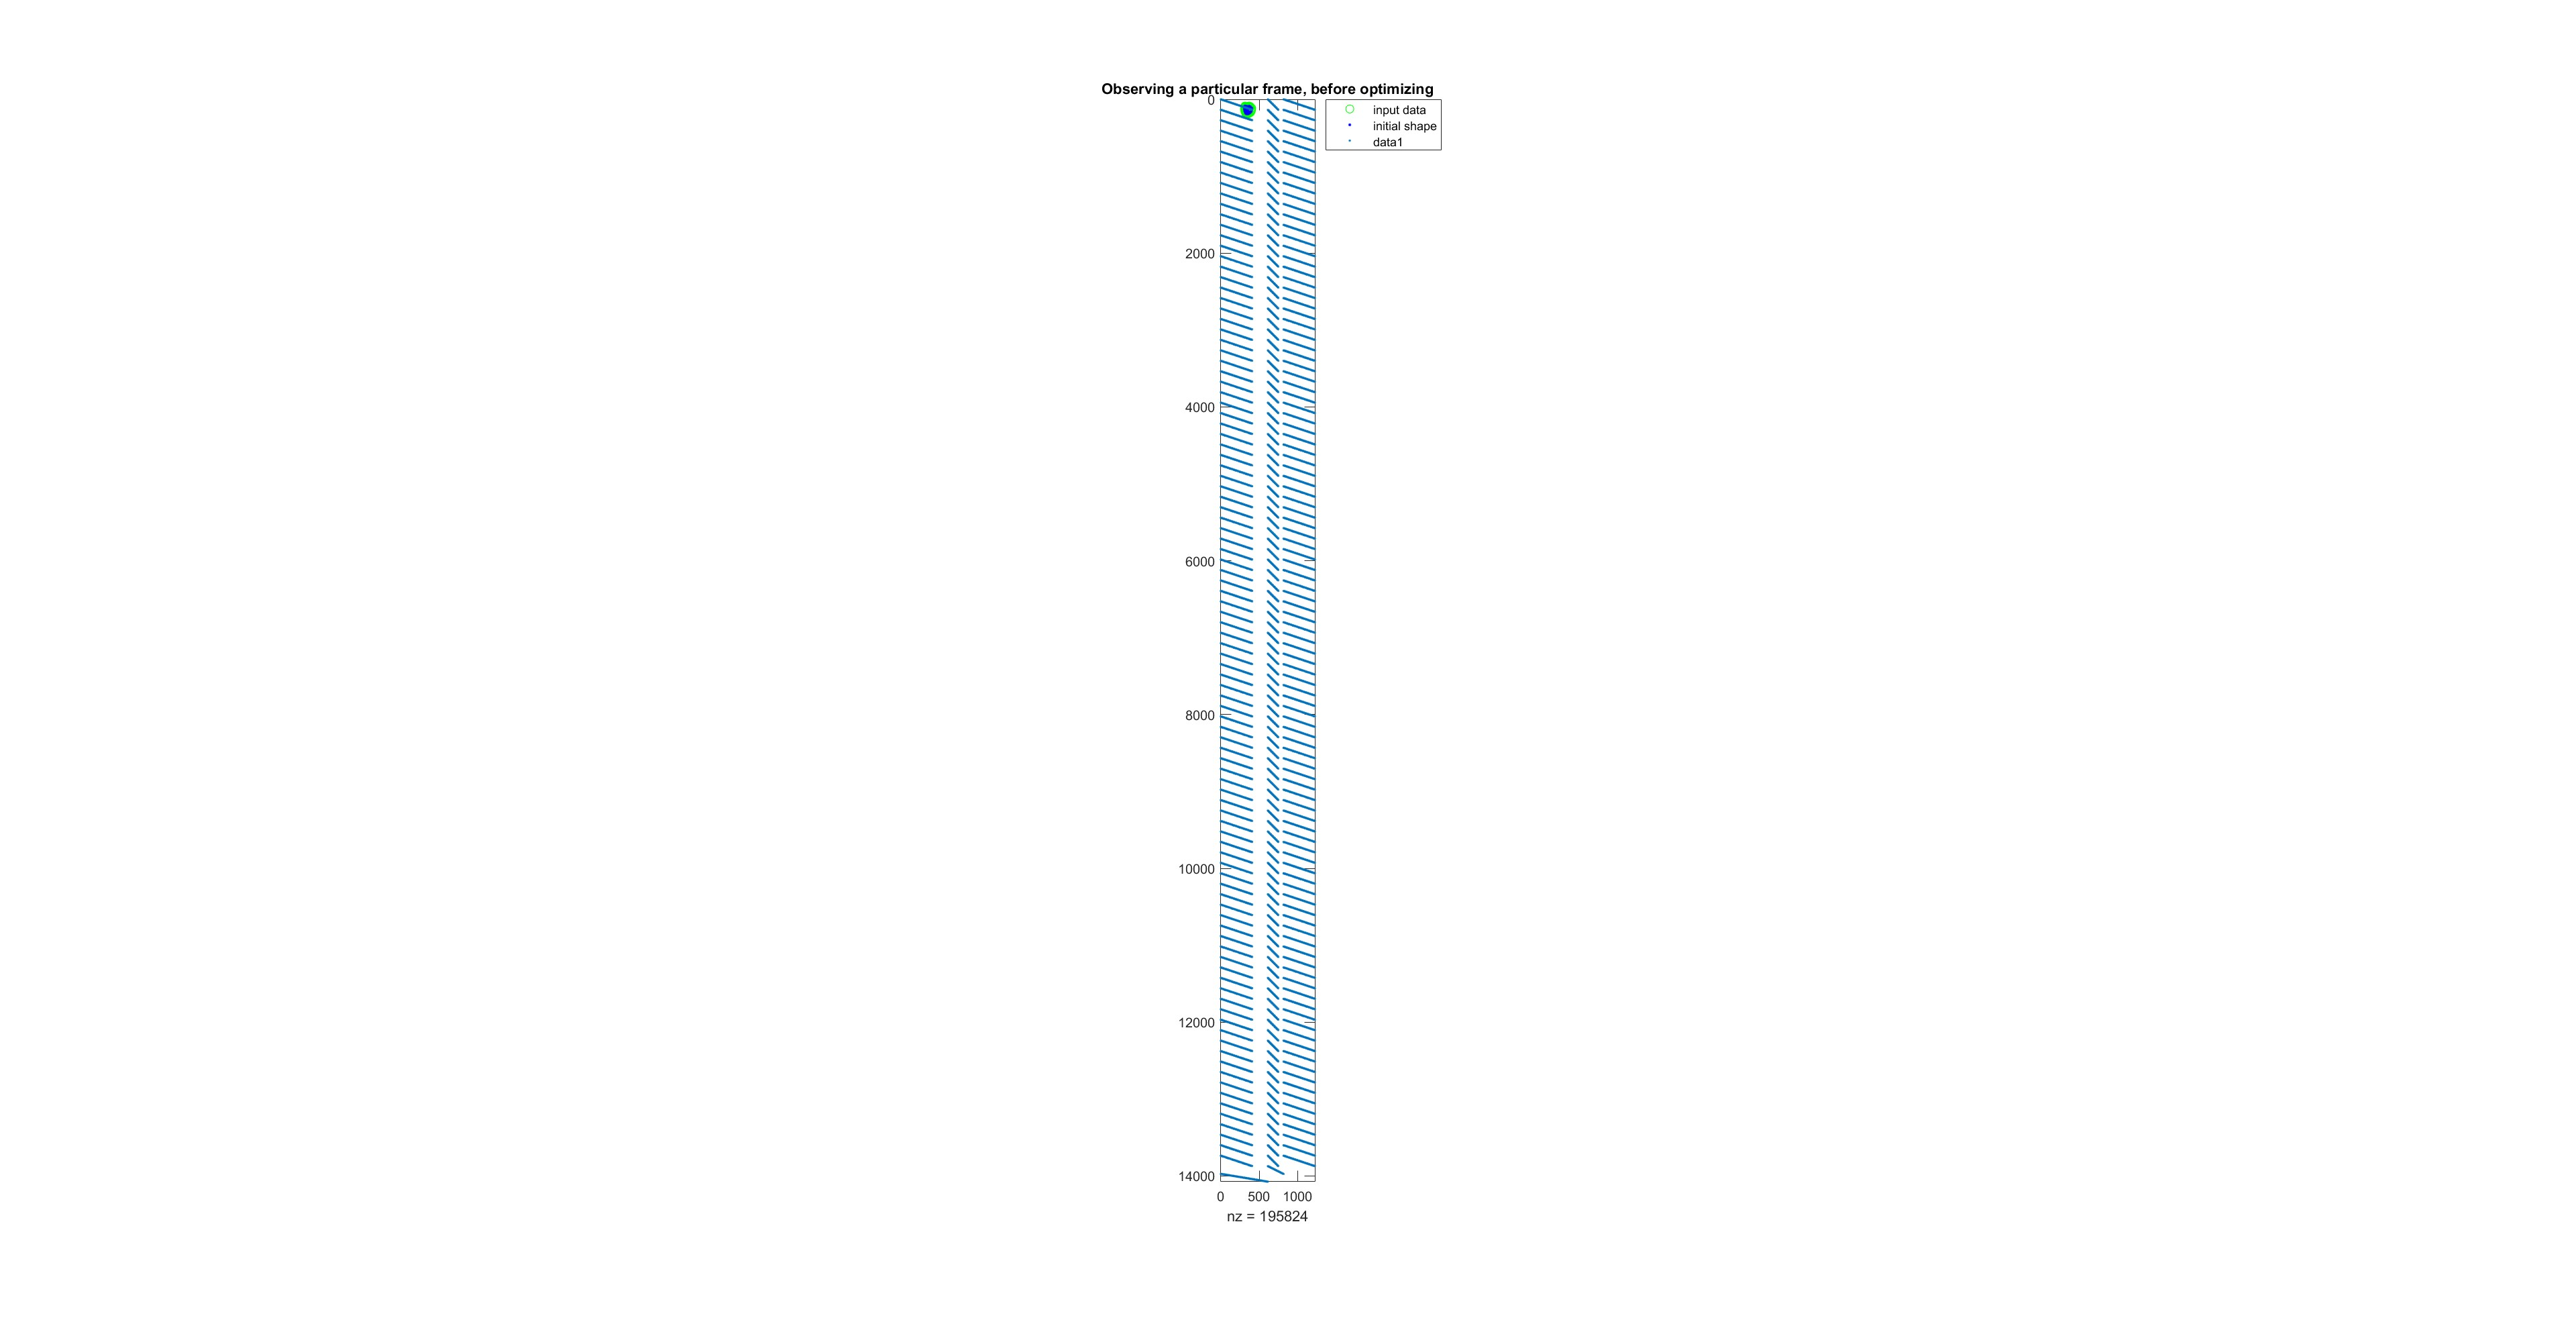
\includegraphics[width=1.0\textwidth]{T2/J}
    \caption{Jacobian result}
    \label{fig:J}
\end{figure}

\subsection{Examples:}
\noindent Here we will show how to reconstruct the human face with the given frames and using the following input parameters:

\begin{itemize}
\item low-rank $K$(it is the number of bases): $2$
\item $camera_prior$(it mean that the $R$ prior is active): $1$
\item $coeff_prior$(it mean that the $L$ prior is active): $1$
\item number of optimizer iterations: $50$
\end{itemize}
\noindent In Figure \ref{fig:coodinates2D} we can see the comparison of the input points of a frame in green against the estimated points of that frame in blue.\\

\begin{figure}[h]
    \centering
    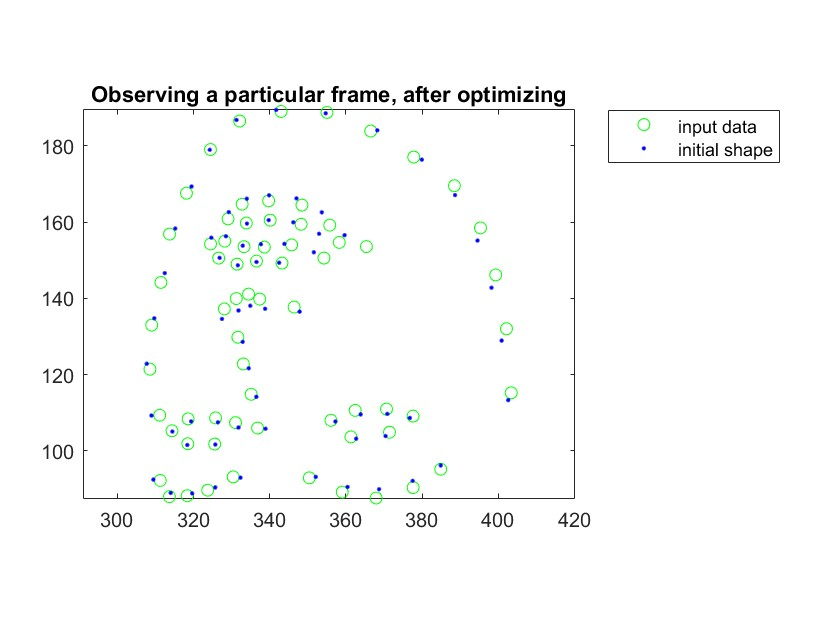
\includegraphics[width=1.0\textwidth]{T2/coodinates2D}
    \caption{Input points compared to optimized points}
    \label{fig:coodinates2D}
\end{figure}

\noindent In Figure \ref{fig:coordinates3D} we can see the estimated 3D points for a frame.\\
\begin{figure}[h]
    \centering
    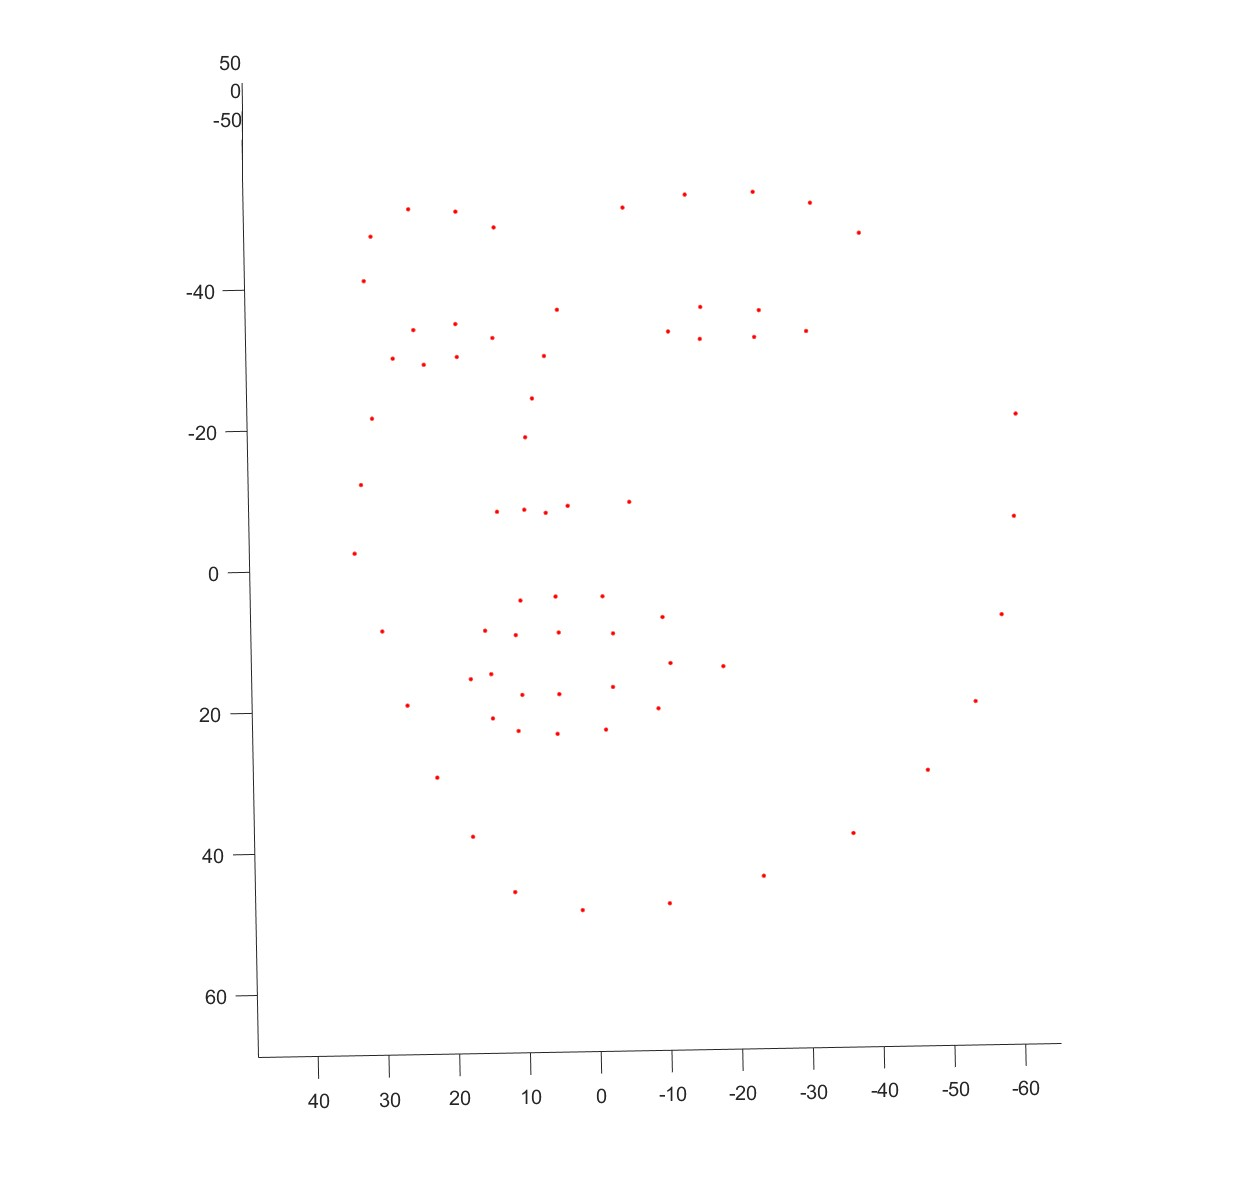
\includegraphics[width=1.0\textwidth]{T2/coordinates3D}
    \caption{3D reconstruction}
    \label{fig:coordinates3D}
\end{figure}
\noindent In Figure \ref{fig:steps} we see the calculation of each of the 50 optimizations, this method has a high cost in performance, but a good result is achieved as shown by the low error at the end.\\
\begin{figure}[h]
    \centering
    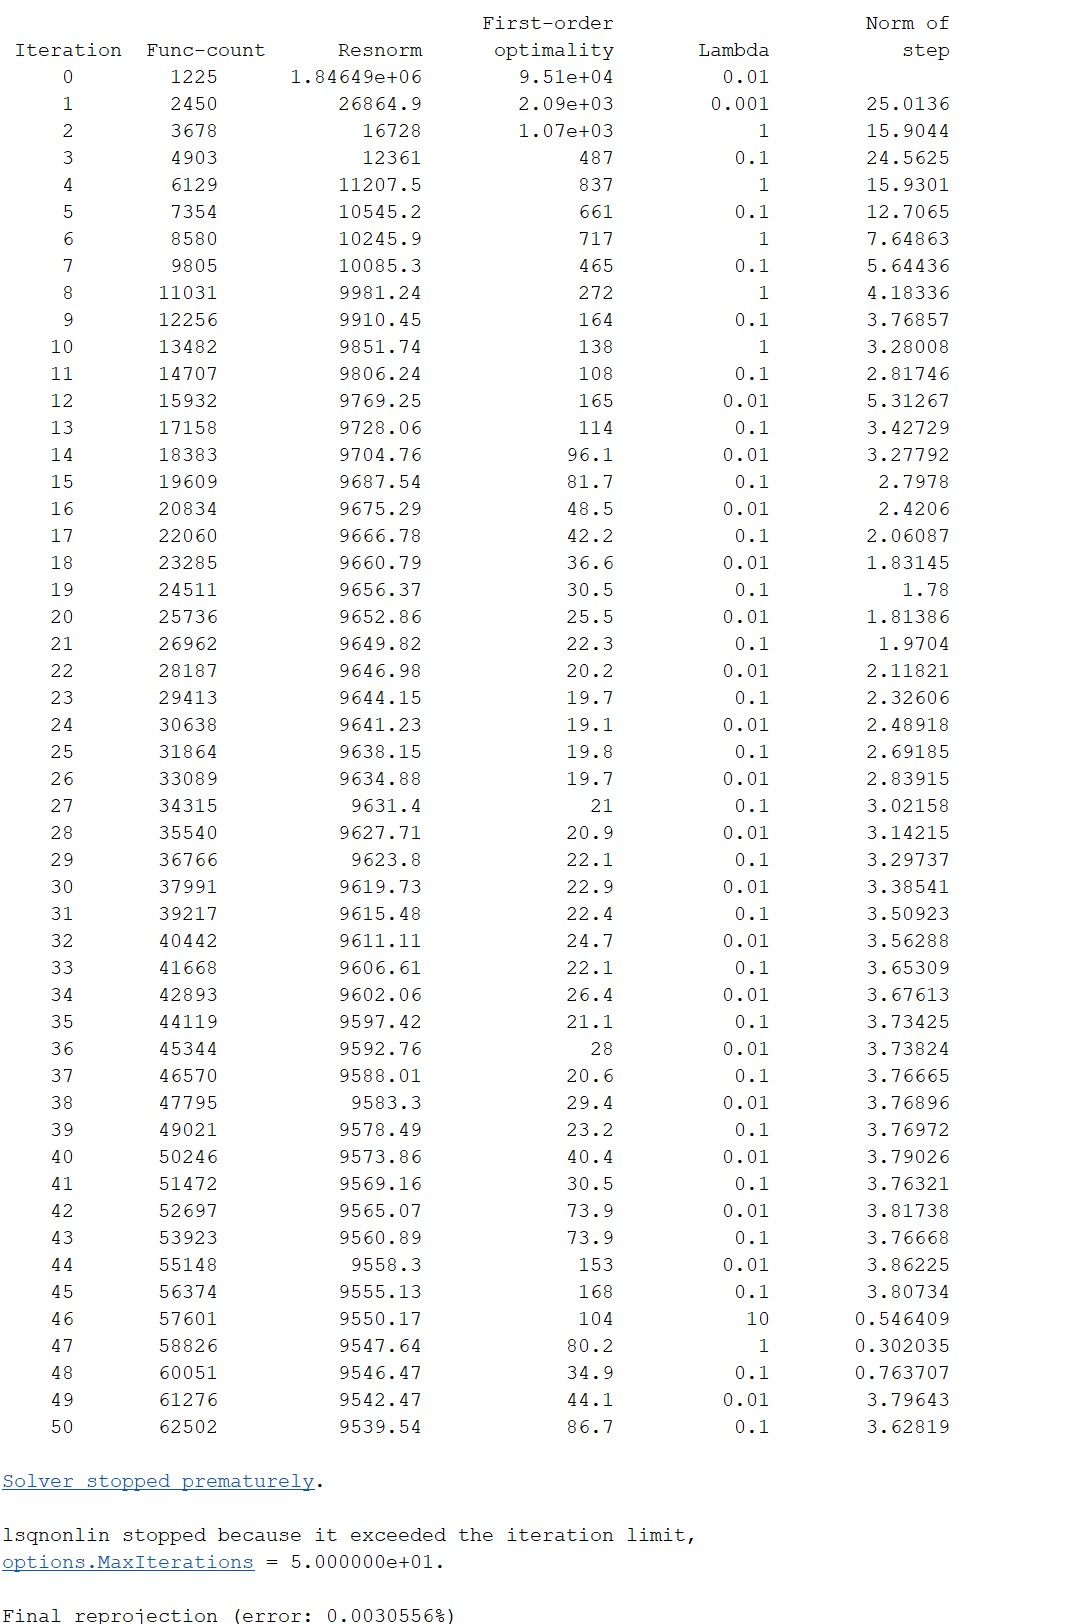
\includegraphics[width=1.0\textwidth]{T2/steps}
    \caption{Optimizer iterations}
    \label{fig:steps}
\end{figure}

\newpage
\section{Third Part (Non-Rigid structure from motion by factorization and assuming a low-rank trajectory model)} 
\noindent In this section, we calculate the reconstruction with the low-rank trajectory method. This method is a little simpler because we already know in advance the matrix of base trajectories, since we defined them with the value of $k$. We will show the structure in Equation \ref{eq:shape_trajectory}.
\begin{equation*}
	\theta=
	\begin{pmatrix}
		\theta_{1}^{1} &  \cdots & \theta_{k}^{1}\\		
		\vdots &  \ddots & \vdots \\
		\theta_{1}^{f} &  \cdots & \theta_{k}^{f}\\		
	\end{pmatrix}_{f\times k}
\end{equation*}
\begin{equation*}
	[a^{x}]=
	\begin{pmatrix}
		a_{11}^{x} &  \cdots & a_{1p}^{x}\\		
		\vdots &  \ddots & \vdots \\
		a_{k1}^{x} &  \cdots & a_{kp}^{x}\\		
	\end{pmatrix}_{k\times p}\text{ , }
	[a^{y}]=
	\begin{pmatrix}
		a_{11}^{y} &  \cdots & a_{1p}^{y}\\		
		\vdots &  \ddots & \vdots \\
		a_{k1}^{y} &  \cdots & a_{kp}^{y}\\		
	\end{pmatrix}_{k\times p}\text{ and }
	[a^{z}]=
	\begin{pmatrix}
		a_{11}^{z} &  \cdots & a_{1p}^{z}\\		
		\vdots &  \ddots & \vdots \\
		a_{k1}^{z} &  \cdots & a_{kp}^{z}\\		
	\end{pmatrix}_{k\times p}
\end{equation*}

\begin{equation}\label{eq:shape_trajectory}	
	\underbrace{\begin{pmatrix}
		x_{1}^{1} & x_{2}^{1} & \cdots & x_{p}^{1}\\
		y_{1}^{1} & y_{2}^{1} & \cdots & y_{p}^{1}\\
		z_{1}^{1} & z_{2}^{1} & \cdots & z_{p}^{1}\\
		\vdots & \vdots & \ddots & \vdots \\
		x_{1}^{f} & x_{2}^{f} & \cdots & x_{p}^{f}\\
		y_{1}^{f} & y_{2}^{f} & \cdots & y_{p}^{f}\\
		z_{1}^{f} & z_{2}^{f} & \cdots & z_{p}^{f}\\
	\end{pmatrix}}_{X}=
	\underbrace{\begin{pmatrix}
		\theta_{f\times k} & 0_{f\times k} & \cdots & 0_{f\times k} \\		
		0_{f\times k} &  \theta_{f\times k} & \vdots & 0_{f\times k}\\
		\vdots &  \vdots &\ddots & \vdots \\
		0_{f\times k} & 0_{f\times k} &  \cdots & \theta_{f\times k}		
	\end{pmatrix}}_{C}
	\underbrace{\begin{pmatrix}
				[a^{x}]_{k\times p} \\		
				[a^{y}]_{k\times p} \\
				[a^{z}]_{k\times p}				
		\end{pmatrix}}_{D}
\end{equation} 
\noindent Where $C$ is called trajectory bases and $D$ is called coefficients.\\

\noindent The low-rank trajectory method is optimized using the factorization method with SVD as shown in the lecture slide in Figure \ref{fig:slideT3}.\\

\begin{figure}[h]
	\centering
	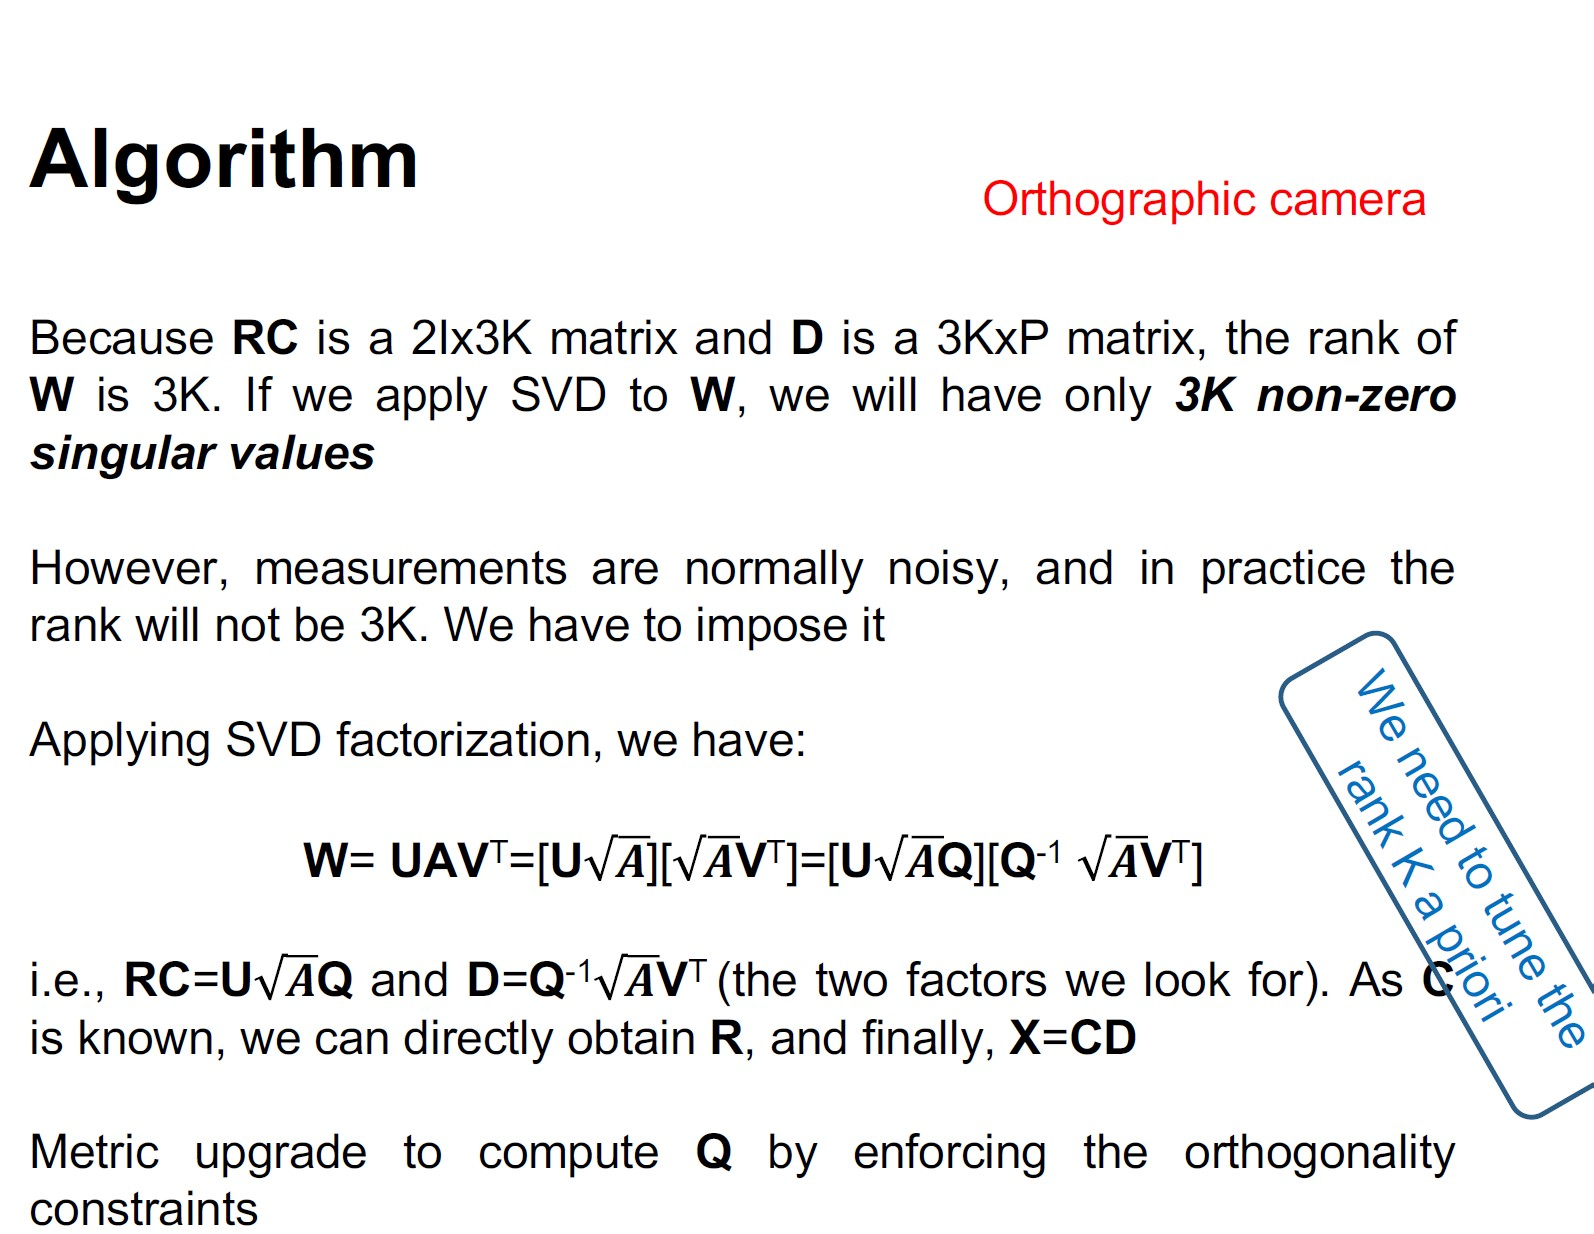
\includegraphics[width=0.55\textwidth]{T3/slide}
	\caption{Factoring slide}
	\label{fig:slideT3}
\end{figure}

\noindent As shown in Figure \ref{fig:slideT3}, in this case, the rank of the matrix $W$ (measurement matrix) is $3k$, since $RC$ has dimensions $2I\times 3k$ and $D$ has dimensions $3k\times p$. Therefore, we should calculate $Q$ by enforcing the orthogonality constraints for $RC$, defined $(RC)(RC)^{'}=I_{2I\times 2I}$, and since $C$ is already known, we can calculate $X$ in the form $X=CD$.\\ 

\subsection{Code:}
\noindent Now we will show how to update $Q$ to find the shape matrix $X$.
\begin{lstlisting}[style=Matlab-editor, numbers=left, caption={Factorization method}, captionpos=b, label={lst:factorization}]
	[U,D,V]=svd(W,0);
	RHat=U(:,1:3*K)*sqrt(D(1:3*K,1:3*K));
	Xhat=sqrt(D(1:3*K,1:3*K))*V(:,1:3*K)';    
	
	% Metric Upgrade step
	[Q] = metricUpgrade(RHat);
	Rsh = RHat*Q;
	% Computing final motion and shape
	R = recoverR(Rsh);
	C = DCT_basis(n_frames,K);
	G = R*C;
	D = inv(G'*G)*G'*W;
	X=C*D;
\end{lstlisting}
\noindent In line 1 in Listing \ref{lst:factorization}, we compute the SVD for $W$ (measurement matrix).\\ 
\noindent In lines 2 and 3 in Listing \ref{lst:factorization}, since we know the rank of the matrix is $3k$, then we restrict the dimensions of the matrices $U$, $D$, and $V$ as follows:
\begin{itemize}
	\item For $U$, we take only its first $3k$ columns.
	\item For $D$, we take only its first $3k$ rows and first 3 columns.
	\item For $V$ we take only the last $3k$ columns
\end{itemize}
\noindent And with these new restrictions for $U$, $D$ and $V$, we calculate the initials matrix $RC=U\sqrt{D}$ and $D=\sqrt{D}V'$.\\
\noindent In line 6 in Listing \ref{lst:factorization}, we update Q by using the orthogonality conditions for the matrix $RHat$, initialized as $RHat=\text{initial } RC$. $Q$ is defined as follows.

\begin{lstlisting}[style=Matlab-editor, numbers=left, caption={Update function}, captionpos=b, label={lst:updatefunct}]
function [Q] = metricUpgrade(LambdaHat,q0)

k = size(LambdaHat,2)/3;
F = size(LambdaHat,1)/2;

if(~exist('q0'))
q0 = zeros(3*k,3);
q0(0*k+1,1) = 1;
q0(1*k+1,2) = 1;
q0(2*k+1,3) = 1;
end
options = optimset('Diagnostics','off','MaxFunEval',100000,'MaxIter',2000,'TolFun',1e-10,'TolX',1e-10);
[q, fval] = fminunc(@evalQ,q0,options,LambdaHat); 

Q = reshape(q,3*k,3);
\end{lstlisting}

\noindent We can see inside the function $metricUpgrade(LambdaHat,q0)$ on line 13 of Listing \ref{lst:updatefunct}, where we compute the $Q$ such that $Q$ minimizes the function $evalQ$ that computes the orthogonality condition.\\ 
\noindent In line 10 in Listing \ref{lst:factorization}, we compute the trajectory bases.\\
\noindent In line 12 in Listing \ref{lst:factorization}, we calculate $D$ from $RC$, solving the equation $\Vert W-RCD\Vert =0$.\\
\noindent In line 13 in Listing \ref{lst:factorization}, finally we calculate the shape matrix $X=CD$.\\
\subsection{Examples:}
\noindent In this part, we show some results of the code for the low-rank trajectory model.\\ 

\noindent We start with the file \textbf{drink\_mocap.mat} that provides the key points whose represent a person is holding a bottle. The inputs for the code are
\begin{itemize}
\item Loaded data: \textbf{drink\_mocap.mat} 
\item Rank of the trajectory basis $K$: 11 
\end{itemize}

\noindent In the Figure \ref{fig:drink}, we can notice the accordance between the truth 3D points and the reconstructed 3D points in a fixed frame $i$ ($\Vert X_{\text{truth shape}}^{i}-X_{\text{reconstructed shape}}^{i}\Vert$).\\
\begin{figure}[h]  
	\centering
	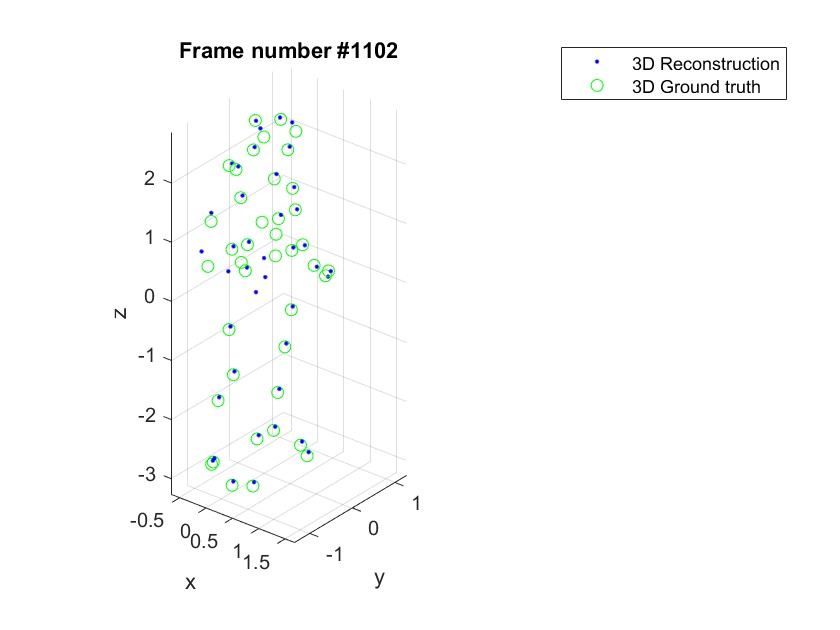
\includegraphics[width=0.7\textwidth]{T3/drink}
	\caption{Comparison between real 3D points (green) and 3D points reconstructed (blue) for \textbf{$drink\_mocap.mat$}.}
	\label{fig:drink}
\end{figure}

\noindent In the Figure \ref{fig:drink_error}, the first error of $0.0034452$ represents the difference between the truth rotation matrix and the reconstructed rotation matrix. The second error of $0.0052503$ represents the difference between the truth shape matrix and the reconstructed shape matrix. 
\begin{figure}[h]
	\centering
	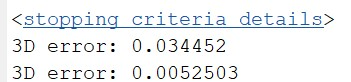
\includegraphics[width=0.4\textwidth]{T3/3DerrorDrink}
	\caption{Error between real points and reconstruction points for \textbf{drink\_mocap.mat}. The first error is for the shape matrix, and the second is for the rotation matrix.}
	\label{fig:drink_error}
\end{figure}
\noindent 

\end{document}          
